% --------------------------------------------------- %
%	Modelo para elaboração do Projeto de Graduação	  %		
%	do curso de Engenharia Elétrica - UFES			  %
%													  %
%	Adaptado do modelo de trabalho acadêmico 'abntex2'%
%	em 27/10/2016									  %
% --------------------------------------------------- %

\documentclass[
	% -- opções da classe memoir --
	12pt,				% tamanho da fonte
	openright,			% capítulos começam em pág ímpar (insere página vazia caso preciso)
	oneside,			% para impressão em recto e verso. Oposto a oneside
	a4paper,			% tamanho do papel. 
	% -- opções da classe abntex2 --
	chapter=TITLE,		% títulos de capítulos convertidos em letras maiúsculas
	%section=TITLE,		% títulos de seções convertidos em letras maiúsculas
	%subsection=TITLE,	% títulos de subseções convertidos em letras maiúsculas
	%subsubsection=TITLE,% títulos de subsubseções convertidos em letras maiúsculas
	% -- opções do pacote babel --
	english,			% idioma adicional para hifenização
	french,				% idioma adicional para hifenização
	spanish,			% idioma adicional para hifenização
	brazil				% o último idioma é o principal do documento
	]{abntex2}

% --------------------------------------------------- %
% 					Pacotes básicos 				  %
% --------------------------------------------------- %
\usepackage{lmodern}			% Usa a fonte Latin Modern			
\usepackage[T1]{fontenc}		% Selecao de codigos de fonte.
\usepackage[utf8]{inputenc}		% Codificacao do documento (conversão automática dos acentos)
\usepackage{lastpage}			% Usado pela Ficha catalográfica
%\usepackage{indentfirst}		% Indenta o primeiro parágrafo de cada seção.
\usepackage{color}				% Controle das cores
\usepackage{graphicx}			% Inclusão de gráficos
\usepackage{microtype} 			% para melhorias de justificação
\usepackage{amsmath}
\usepackage[table,xcdraw]{xcolor} 
\usepackage{multirow}			% Para usar a tabela gerada no www.tablesgenerator.com
\usepackage{lscape} %serve para inserir página no modo paisagem
\usepackage{pdflscape} %serve para inserir página no modo paisagem
\usepackage{subfig}
\usepackage{subfloat}
% >> Pacotes de citações
\usepackage[brazilian,hyperpageref]{backref}	 % Paginas com as citações na bibl
\usepackage[alf]{abntex2cite}	% Citações padrão ABNT
\usepackage{url}
% >> Configuração dos pacotes de citações
	% ---
	% Configurações do pacote backref
	% Usado sem a opção hyperpageref de backref
	\renewcommand{\backrefpagesname}{Citado na(s) página(s):~}
	% Texto padrão antes do número das páginas
	\renewcommand{\backref}{}
	% Define os textos da citação
	\renewcommand*{\backrefalt}[4]{
		\ifcase #1 %
			Nenhuma citação no texto.%
		\or
			Citado na página #2.%
		\else
			Citado #1 vezes nas páginas #2.%
		\fi}%
 
% >>> Insere a pasta onde estão contidas as figuras <<<
\graphicspath{{imagens/}}

% --------------------------------------------------- %
%		Redefinição e criação de comandos 			  %
% --------------------------------------------------- %
	
% >>> Mudar tamanho da fonte dos capítulos <<<
\renewcommand*{\chapnumfont}{\normalfont\large\bfseries\sffamily}
\renewcommand*{\chaptitlefont}{\normalfont\large\bfseries\sffamily}

\usepackage{titlesec}
\titleformat{\section}
  {\normalfont\normalsize\bfseries}{\thesection}{1em}{}
\titleformat{\subsection}
  {\normalfont\normalsize\bfseries}{\thesubsection}{1em}{}

% >>> Mudar tamanho da fonte das legendas <<<
\usepackage[font=footnotesize]{caption}

% >>> Definição do tipo CRONOGRAMA <<<
% e.g.:
% \begin{cronograma}[!h]
% 		Insira o cronograma aqui! (tabela)
% \eng{cronograma}
\newcommand{\cronogramaname}{Cronograma}
\newcommand{\listofcronogramasname}{Lista de Cronogramas}

\newfloat[chapter]{cronograma}{loc}{\cronogramaname}
\newlistof{listofcronogramas}{loc}{\listofcronogramasname}
\newlistentry{cronograma}{loc}{0}

\counterwithout{cronograma}{chapter}
\renewcommand{\cftcronogramaname}{\cronogramaname\space} 
\renewcommand*{\cftcronogramaaftersnum}{\hfill--\hfill}

% >>> Definição do tipo QUADRO <<<
% e.g.:
% \begin{quadro}[!h]
%  Insira aqui o quadro (tabela)
% \end{quadro} 
\newcommand{\quadroname}{Quadro}
\newcommand{\listofquadrosname}{Lista de Quadros}

\newfloat[chapter]{quadro}{loq}{\quadroname}
\newlistof{listofquadros}{loq}{\listofquadrosname}
\newlistentry{quadro}{loq}{0}

\counterwithout{quadro}{chapter}
\renewcommand{\cftquadroname}{\quadroname\space} 
\renewcommand*{\cftquadroaftersnum}{\hfill--\hfill}

% >>> Comando para inserir a fonte em figuras <<<
% e.g.:
% \begin{figure}[!h]
%	\centering
%	\caption{Legenda da Figura.}
%	\includegraphics[width=0.7\textwidth]{figura.jpg}
%	\source[\citeonline{Referencia}.]
%	\label{fig:label_da_figura}
%  \end{figure}
%
% Obs.: Se utilizar apenas "\source", será inserido
%       "Produção do próprio autor."

\newcommand{\source}[1][Produção do próprio autor.]{\begin{flushleft}\footnotesize Fonte: #1\end{flushleft}}

% --------------------------------------------------- %
%		Informações para personalização da capa		  %
% --------------------------------------------------- %
\newcommand{\universidade}{Universidade Federal do Espírito Santo}
\newcommand{\centro}{Centro Tecnológico}
\newcommand{\departamento}{Departamento de Engenharia Elétrica}
\newcommand{\disciplina}{Projeto de Graduação}
\newcommand{\imprimirINSTITUICAO}{
	\MakeUppercase{\universidade} \\
	\MakeUppercase{\centro} \\
	\MakeUppercase{\departamento} \\
	\MakeUppercase{\disciplina} \\
}
% --------------------------------------------------- %
%		Informações para capa e folha de rosto		  %
% --------------------------------------------------- %
\titulo{Automação de Emprétimos de Equipamentos do Laboratório}
\autor{Lucas Soares Pessini}
\local{Vitória-ES}
\data{Junho/2019}
\orientador{Prof. Dr. André Ferreira}
\coorientador{Profa. Dra. Carla César Martins Cunha}
\instituicao{%
	\universidade
  	\par
	\centro
  	\par
	\departamento
	\par
	\disciplina
	\par}
\tipotrabalho{Projeto de Graduação}
% O preambulo deve conter o tipo do trabalho, o objetivo, 
% o nome da instituição e a área de concentração 
\preambulo{Parte manuscrita do Projeto de Graduação do aluno \imprimirautor, apresentado ao Departamento de Engenharia Elétrica do Centro Tecnológico da Universidade Federal do Espírito Santo, como requisito parcial para obtenção do grau de Engenheiro Eletricista.}

% --------------------------------------------------- %
%		Configurações do aspecto final do PDF		  %
% --------------------------------------------------- %
% >> Alterando o aspecto da cor azul
\definecolor{blue}{RGB}{41,5,195}
% Informações do PDF
\makeatletter
\hypersetup{
     	%pagebackref=true,
		pdftitle={\@title}, 
		pdfauthor={\@author},
    	pdfsubject={\imprimirpreambulo},
	    pdfcreator={LaTeX with abnTeX2},
		pdfkeywords={abnt}{latex}{abntex}{abntex2}{trabalho acadêmico}, 
		colorlinks=true,       		% false: boxed links; true: colored links
    	linkcolor=black,          	% color of internal links
    	citecolor=black,        		% color of links to bibliography
    	filecolor=magenta,      		% color of file links
		urlcolor=black,
		bookmarksdepth=4
}
\makeatother

% --------------------------------------------------- %
%		Espaçamentos entre linhas e parágrafos 		  %
% --------------------------------------------------- %
% >> O tamanho do parágrafo é dado por:
\setlength{\parindent}{0cm}
% >> Controle do espaçamento entre um parágrafo e outro:
\setlength{\parskip}{18pt}

% --------------------------------------------------- %
%				Compila o Índice 					  %
% --------------------------------------------------- %
\makeindex

% --------------------------------------------------- %
%				Início do Documento					  %
% --------------------------------------------------- %

\begin{document}

% >>> Seleciona o idioma do documento (conforme pacotes do babel)
% \selectlanguage{english}
\selectlanguage{brazil}

% >>> Retira espaço extra obsoleto entre as frases.
\frenchspacing 

% --------------------------------------------------- %
%				Elementos Pré-Textuais				  %
% --------------------------------------------------- %
% \pretextual

% --------------------------------------------------- %
%						Capa						  %
% --------------------------------------------------- %
% >>> Capa Personalizada
\renewcommand{\imprimircapa}{%
	\begin{capa}%
		\center
		{\ABNTEXchapterfont\bfseries\large\imprimirINSTITUICAO}
			\vspace*{1.5cm}
		\includegraphics*[width=0.25\textwidth]{brasao_ufes.jpg}
			\vspace*{1.5cm} \\
		{\ABNTEXchapterfont\Large\imprimirautor}
				\vspace*{2.5cm} \\
		{\ABNTEXchapterfont\bfseries\Large\imprimirtitulo}
			\vfill
			\vspace*{0.5cm}
		{\large\imprimirlocal}
		\par
		{\large\imprimirdata}
			\vspace*{1cm}
	\end{capa}
}

\imprimircapa

% --------------------------------------------------- %
%					Folha de Rosto 					  %
% --------------------------------------------------- %
% >> O * indica que haverá a ficha bibliográfica

\renewcommand{\imprimirfolhaderosto}{

\begin{folhaderosto}
	\begin{center}
    	{\ABNTEXchapterfont\large\imprimirautor}
		    \vspace*{\fill}\vspace*{\fill}
    	\begin{center}
	    	\ABNTEXchapterfont\bfseries\Large\imprimirtitulo
	    \end{center}
    		\vspace*{\fill}
    		\hspace{.45\textwidth}
	    \begin{minipage}{.5\textwidth}
        	\imprimirpreambulo
	    \end{minipage}
    		\vspace*{\fill}
	    \end{center}  
        \begin{center}
        	% >> Se necessáiro, ajustar os \vspace
        	%\vspace*{0.5cm}
        {\large\imprimirlocal}
        \par
        {\large\imprimirdata}
       		%\vspace*{1cm}
      \end{center}
\end{folhaderosto}
}

\imprimirfolhaderosto

% --------------------------------------------------- %
%					Ficha Catalográfica 			  %
% --------------------------------------------------- %

% Isto é um exemplo de Ficha Catalográfica, ou ``Dados internacionais de
% catalogação-na-publicação''. Você pode utilizar este modelo como referência. 
% Porém, provavelmente a biblioteca da sua universidade lhe fornecerá um PDF
% com a ficha catalográfica definitiva após a defesa do trabalho. Quando estiver
% com o documento, salve-o como PDF no diretório do seu projeto e substitua todo
% o conteúdo de implementação deste arquivo pelo comando abaixo:
%
% \begin{fichacatalografica}
%     \includepdf{fig_ficha_catalografica.pdf}
% \end{fichacatalografica}

%\begin{fichacatalografica}
%	\sffamily
%	\vspace*{\fill}					% Posição vertical
%	\begin{center}					% Minipage Centralizado
%	\fbox{\begin{minipage}[c][8cm]{13.5cm}		% Largura
%	\small
%	\imprimirautor
%	%Sobrenome, Nome do autor
%	
%	\hspace{0.5cm} \imprimirtitulo  / \imprimirautor. --
%	\imprimirlocal, \imprimirdata-
%	
%	\hspace{0.5cm} \pageref{LastPage} p. : il. (algumas color.) ; 30 cm.\\
%	
%	\hspace{0.5cm} \imprimirorientadorRotulo~\imprimirorientador\\
%	
%	\hspace{0.5cm}
%	\parbox[t]{\textwidth}{\imprimirtipotrabalho~--~\imprimirinstituicao,
%	\imprimirdata.}\\
%	
%	\hspace{0.5cm}
%		1. Palavra-chave1.
%		2. Palavra-chave2.
%		2. Palavra-chave3.
%		I. Orientador.
%		II. Universidade xxx.
%		III. Faculdade de xxx.
%		IV. Título 			
%	\end{minipage}}
%	\end{center}
%\end{fichacatalografica}

% --------------------------------------------------- %
%					Folha de Aprovação			      %
% --------------------------------------------------- %
% >>> Após apresentação do trabalho, substitua todo o conteúdo 
% por uma imagem da página assinada pela banca com o comando abaixo:
% \includepdf{folhadeaprovacao_final.pdf}

\begin{folhadeaprovacao}
  \begin{center}
    {\ABNTEXchapterfont\large\imprimirautor}
	\begin{center}
     	\ABNTEXchapterfont\bfseries\Large\imprimirtitulo
    \end{center}
    %\vspace*{\fill}
  \end{center}    
    \imprimirpreambulo
		\vspace{-0.5cm}
    \begin{center}
		\hspace{.45\textwidth}
    \begin{minipage}{.5\textwidth}
        Aprovado em ??, de Dezembro de 2016. \\\\
        \textbf{COMISSÃO EXAMINADORA:}
        \assinatura{\textbf{\imprimirorientador} \\ Instituto Federal do Espírito Santo \\ Orientadora} 
        \assinatura{\textbf{\imprimircoorientador} \\ Universidade Federal do Espírito Santo \\ Coorientadora}
		\assinatura{\textbf{Profa. Dra. Fulana} \\ Universidade Federal do Espírito Santo \\ Examinador}
		\assinatura{\textbf{Prof. Dr. Fulano} \\ Universidade Federal do Espírito Santo \\ Examinador}
    \end{minipage}
	    \vspace*{\fill}
   \end{center}
         
   \begin{center}
      	% >> Se necessáiro, ajustar os \vspace
		%\vspace*{0.5cm}
    	{\large\imprimirlocal}
    	\par
    	{\large\imprimirdata}
   		%\vspace*{1cm}
  \end{center}  
\end{folhadeaprovacao}

% --------------------------------------------------- %
%						Dedicatória				      %
% --------------------------------------------------- %
\begin{dedicatoria}
   \vspace*{\fill}
   \centering
   \noindent
   \textit{ Insira a dedicatória aqui!
   } \vspace*{\fill}
\end{dedicatoria}

% --------------------------------------------------- %
%					Agradecimentos				      %
% --------------------------------------------------- %

\begin{agradecimentos}
	Insira os agradecimentos aqui!
\end{agradecimentos}

% --------------------------------------------------- %
%						Epígrafe			      	  %	
% --------------------------------------------------- %

\begin{epigrafe}
    \vspace*{\fill}
	\begin{flushright}
		Insira a epígrafe aqui!
	\end{flushright}
\end{epigrafe}

% --------------------------------------------------- %
%						Resumo				      	  %	
% --------------------------------------------------- %

% Resumo em português
\setlength{\absparsep}{18pt} % ajusta o espaçamento dos parágrafos do resumo
\begin{resumo}

Insira o resumo aqui!

\textbf{Palavras-chave}: Palavra-chave 1; Palavra-chave 2; ...; Palavra-chave N.
\end{resumo}

%% resumo em inglês
%\begin{resumo}[Abstract]
% \begin{otherlanguage*}{english}
%   \noindent 
%   \textbf{Keywords}: latex. abntex. text editoration.
% \end{otherlanguage*}
%\end{resumo}
 
% --------------------------------------------------- %
%					Lista de Figuras	      	  	  %	
% --------------------------------------------------- %
\renewcommand{\listfigurename}{Lista de Figuras}
\listoffigures*
\cleardoublepage

% --------------------------------------------------- %
%					Lista de Tabelas				  %	
% --------------------------------------------------- %

\pdfbookmark[0]{\listtablename}{lot}
\listoftables*
\cleardoublepage

% --------------------------------------------------- %
%					Lista de Quadros				  %	
% --------------------------------------------------- %

\pdfbookmark[0]{\listofquadrosname}{loq}
\listofquadros*
\cleardoublepage

% --------------------------------------------------- %
%			Lista de Abreviaturas e Siglas			  %	
% --------------------------------------------------- %
\begin{siglas}
  \item[UFES] \textit{Universidade Federal do Espírito Santo}
\end{siglas}

% --------------------------------------------------- %
%					Lista de Símbolos				  %	
% --------------------------------------------------- %

\begin{simbolos}
	\item[]
\end{simbolos}

% --------------------------------------------------- %
%						Sumário						  %	
% --------------------------------------------------- %

\pdfbookmark[0]{\contentsname}{toc}
\tableofcontents*
\cleardoublepage

% --------------------------------------------------- %
%					Elementos Textuais				  %
% --------------------------------------------------- %

\textual

\chapter[Introdução]{Introdução}
% Ajustar esse \vspace de acordo com o necessário
\vspace{-42pt}

Teste de citação: \cite{DepEngEle}

\chapter[Justificativa]{Justificativa}
% Ajustar esse \vspace de acordo com o necessário
\vspace{-42pt}
Como a DAELN possui equipamentos de alto custo, é necessário ter um controle minimamente estruturado dos empréstimos. Para ter este controle, os dados do equipamento e o aluno que solicitou ser armazenado corretamente para que, caso ocorra algum problema com o equipamento, sejam tomadas atitudes necessárias para resolvê-lo. O controle manual desses empréstimos é efetivo até certo ponto, mas pode apresentar alguns erros.

Com um sistema automatizado para ganhar agilidade, maior segurança na data do empréstimo e ainda manter um histórico atualizado de cada um dos equipamentos de empréstimos. Uma implementação de um sistema eletrônico para controlar os empréstimos necessários para que os dados sejam registrados corretamente, e isso acabará evitando tempestades no futuro.

Manter um histórico de empréstimos é importante para evitar o uso excessivo do mesmo equipamento, ou seja, nem sempre emprestar equipamentos mesmo para evitar o seu desgaste excesivo.Como uso já foi dito antes, até que existam sistemas que possam ser utilizados, mas eles não são desenvolvidos para isto, possuindo funções excedentes e alto custo. Desta forma, o sistema foi desenvolvido para automatizar o processamento de empréstimos do equipamento e armazenar o histórico do mesmo.

\chapter[Objetivos]{Objetivos}
% Ajustar esse \vspace de acordo com o necessário
\vspace{-42pt}
\section[Objetivos Geral]{Objetivos Geral}
O objetivo geral deste trabalho é o desenvolvimento de um sistema de controle para equipamentos dos Laboratórios da Engenharia Elétrica da Ufes. Este sistema obtém, a partir de informações de dados, a data do produto (patrimonial) e o estudante (RA), informações adicionais adicionais de continuação de propriedades.

O projeto em desenvolvimento para a disciplina de Projeto Orientado tem como objetivo a resolução de alguma problemática cotidiana por vias de Internet das coisas (do inglês, Internet of Things - IoT)[1][3]. Tomando como base a ideia acordada pelo professor e alunos da disciplina, o grupo propôs desenvolver um projeto que apresente melhorias em economia de tempo e trabalho humano dos laboratórios de eletrônica do prédio do CT II. 

Tais laboratórios são constantemente utilizados e, dessa forma, o grupo se propôs a pensar em uma solução e executá-la de forma que auxilie o processo de gerenciamento de KITs dos laboratórios, ajudando tanto alunos e professores como os próprios funcionários do local. A ideia tem aplicabilidade em diversas instâncias, para tanto, tal ideia foi generalizada para gerenciamento de KITs, de forma a atender outras áreas e não somente os laboratórios do CT II. 

Atualmente os Kits ficam armazenados no almoxarifado do laboratório e quando são emprestados é preciso que o aluno entregue algum documento com foto (Carteira de Identidade ou Carteira Estudantil) onde o funcionário do laboratório guarda o documento junto com uma ficha, sendo entregue somente quando o estudante devolver o KIT. Isso gera confusão para ser pegar e entregar dos documentos e demora com filas de estudantes. Por isso é necessário que seja feito um controle mais aprimorado desses empréstimos.Além disso, o sistema manual não gurada o histórico de empréstimo dos equipamentos. 

O projeto proposto tem como objetivo geral a simplificação e automatização do gerenciamento de empréstimos de livros e equipamentos em bibliotecas e empresas. Como objetivos específicos temos o intuito de registrar toda uma coleção de KITs didáticos para aulas de eletrônica nos laboratórios do CT II e ter controle com um cadastro de usuários.
Um sistema automatizado se ganha agilidade, maior segurança nos dados do empréstimo e ainda mantém um histórico sempre atualizado dos empréstimos de cada KIT.


\section[Objetivos Específicos]{Objetivos Especificos}
A automatização de empréstimos pode ser feita com algum sistema já existente, mas os sistemas são desenvolvidos para gerenciamento de bibliotecas[6], o que faz com que eles possuam funções que não são necessárias no caso de controle de empréstimos de equipamentos. Os objetivos específicos desse projeto foram divididos em alguns tópicos, os quais estão listados nos tópicos a seguir:

\begin{itemize}
   \item Desenvolver um software na linguagem C para fazer a leitura dos códigos de barra do RA e do patrimônio do equipamento por meio de um leitor conectado a Raspberry Pi;
   \item Modelar um sistema de banco de dados, o qual irá armazenar os dados dos empréstimos;
   \item Desenvolver uma interface web para fazer o controle dos empréstimos de maneira automatizada. Através dessa interface, o usuário poderá controlar todo o sistema e terá acesso a todos os relatórios desejados;
   \item Desenvolver uma forma de integração entre a interface web e o software que faz as
leituras dos códigos de barra;
   \item Fazer as verificações necessárias no sistema e por fim validar o seu funcionamento;
   \item Com o sistema funcionando, desenvolver um script para a sua instalação;
   \item Desenvolver um manual de operação do sistema para fornecer para o usuário.
\end{itemize}


\chapter[Metodologia]{Metodologia}
% Ajustar esse \vspace de acordo com o necessário
\vspace{-42pt}
Na parte de hardware, teremos que utilizar:
\begin{itemize}
   \item O servidor do LCEE que fará a armazenagem e processamento de dados; 
   \item Um leitor de RFID para registrar o login do usuário;
   \item Arduíno para viabilizar a comunicação do leitor RFID com o servidor;
   \item Tranca eletrônica para segurança dos equipamentos/KITs.
\end{itemize}
Já na parte de software podemos utilizar:
\begin{itemize}
   \item Um Framework PHP como o Laravel ou CakePHP para facilitar no desenvolvimento do sistema de login; 
   \item Banco de dados SQL (Structured Query Language).
\end{itemize}

Uma inspiração que temos para software é a plataforma web Lend-Itens. Abaixo podemos ver como ficará a plataforma Web:

\begin{figure}[!h]
	\centering
	\caption{Na plataforma Lend-Itens, os usuários podem acessar sua biblioteca para pesquisar um item e reservá-lo, bem como ver seu histórico e os empréstimos atuais.}
	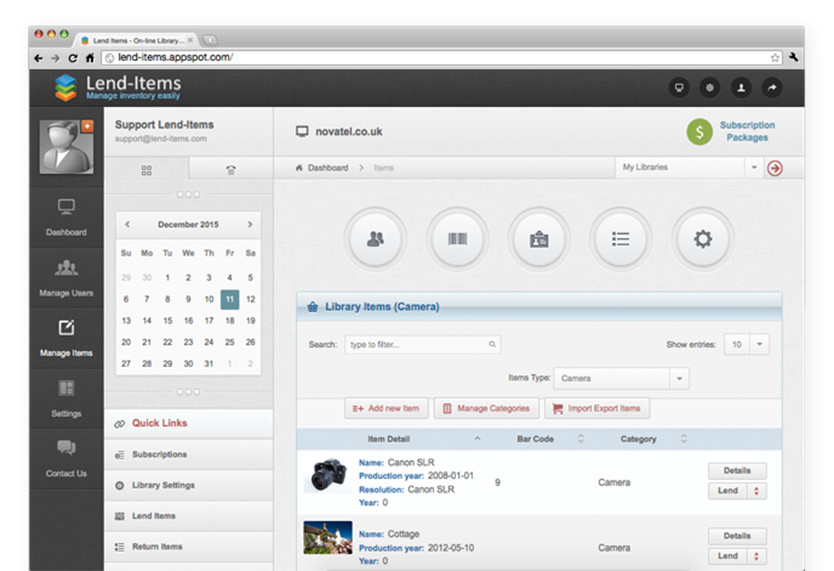
\includegraphics[width=0.7\textwidth]{figura1.jpg}
	\source[\citeonline{DepEngEle}.]
	\label{fig:label_da_figura}
\end{figure}


\begin{figure}[!h]
	\centering
	\caption{Pode-se verificar quais são as pessoas que utilizam a plataforma.}
	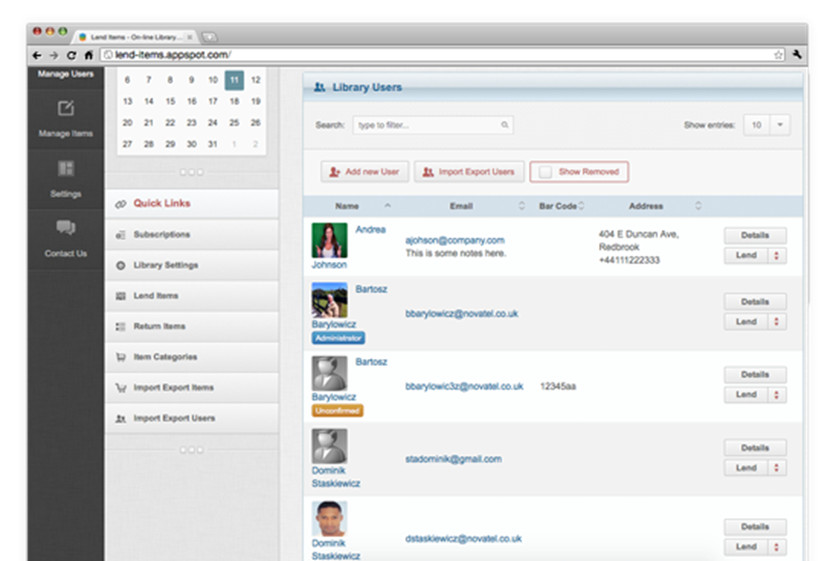
\includegraphics[width=0.7\textwidth]{figura2.jpg}
	\source[\citeonline{DepEngEle}.]
	\label{fig:label_da_figura}
\end{figure}

Outras plataformas que podemos ter como base são Vaivem, apresentando a seguinte interface:

\begin{figure}[!h]
	\centering
	\caption{Interface de Vaivem.}
	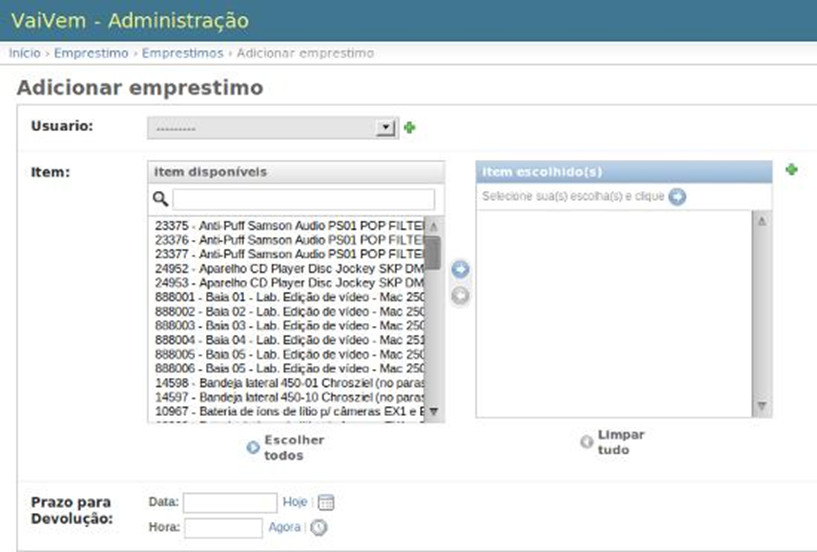
\includegraphics[width=0.7\textwidth]{figura3.jpg}
	\source[\citeonline{DepEngEle}.]
	\label{fig:label_da_figura}
\end{figure}


Há outros softwares também como Software de Controle de UPJ e TotalLoc.
Também estamos utilizando o seguinte modelo de banco de dados para nosso projeto :
\begin{figure}[!h]
	\centering
	\caption{Configuração do Banco de Dados.}
	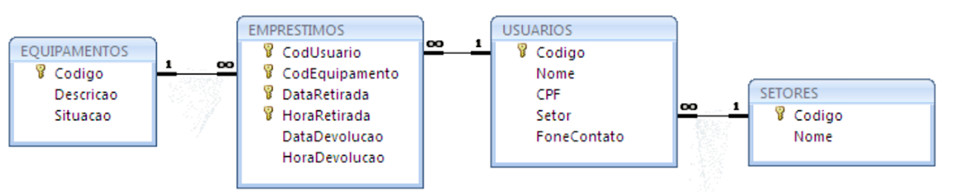
\includegraphics[width=0.7\textwidth]{figura4.jpg}
	\source[\citeonline{DepEngEle}.]
	\label{fig:label_da_figura}
\end{figure}


Também podemos ver quando o banco é acessado pelo seguintes esquemático:

\begin{figure}[!h]
	\centering
	\caption{Acesso do Banco de Dados.}
	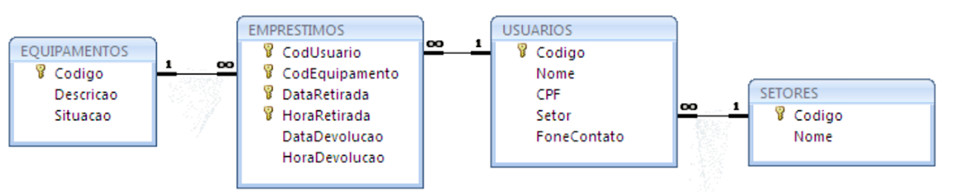
\includegraphics[width=0.7\textwidth]{figura4.jpg}
	\source[\citeonline{DepEngEle}.]
	\label{fig:label_da_figura}
\end{figure}


% --------------------------------------------------- %
%				Elementos Pós-Textuais				  %
% --------------------------------------------------- %

\postextual

% --------------------------------------------------- %
%				Referências Bibliográficas		      %
% --------------------------------------------------- %

\bibliographystyle{abntex2-alf} % Autor-Data
\renewcommand{\bibname}{Referências Bibliográficas}
\bibliography{bibliografia}

% --------------------------------------------------- %
%						Apêndices				  	  %
% --------------------------------------------------- %

\begin{apendicesenv}
% Imprime uma página indicando o início dos apêndices
\partapendices

% Insira os apêndices aqui em forma de capítulos

\end{apendicesenv}

% --------------------------------------------------- %
%						Anexos						  %
% --------------------------------------------------- %

\begin{anexosenv}
%
%% Imprime uma página indicando o início dos anexos
\partanexos

\end{anexosenv}

% --------------------------------------------------- %
%					Índice Remissivo				  %
% --------------------------------------------------- %
\phantompart
\printindex

\end{document}
